\clearpage
% \setcounter{page}{1}
% \maketitlesupplementary

\appendix
\section{Practical quantum copmutation}
The purpose of this section is to provide the reader with the minimal understanding of quantum information, processes and errors.
Although quantum computation lives in Hilbert space, for this appendix we will omit that by assuming the space of complex numbers.
Readers familiar with quantum computation may skip this part.

\subsection{Information}
Quantum systems that are subject to noise are described by a density operator, which is represented as a matrix.
\begin{definition} (density matrix - loose)
The density matrix $\rho\in\mathbb{C}^{2^n\times 2^n}$ decsribing a $n$-qubit system is positive semi-definite with unit trace.
That is, for every eigenvalue $\lambda_i$ of $\rho$: $\lambda_i\in\mathbb{R}$ and $\lambda_i\geq 0$ with $\sum_i \lambda_i=1.$
\end{definition}

\noindent Additionally when a state $\rho$ is coupled with the environment is called \textit{mixed}, otherwise is refered to as \textit{pure} and it satisfies $\rho^2=\rho$ (i.e. a projector).

At this point it should be obvious that a full-state simulation of a quantum system is difficult due to the exponential scaling of the state.
Nevertheless, there are thechniques that \cite{waintal2026competequantumcomputerslecture,PhysRevLett.128.220503} are efficient in regimes with low correlations.

\subsection{Computation}
\label{sec:computation}
Computation is realized through quantum processes, which in the ideal case are unitary maps

\begin{definition} (unitary process)
\label{def:unitary}
A $n$-qubit state $\rho$ is evolved under the unitary transformation as
\begin{equation}
    \mathcal{U}(\rho) = U\rho U^\dagger
\end{equation}
where $U\in\mathbb{C}^{2^n\times 2^n}$ with $U^{-1}=U^\dagger$ and $\cdot^\dagger$ denoting the conjugate-transpose.
\end{definition}

In practise, such processes couple the system with the environment leading to loss of coherence withing the computational states.
Such noisy processes (or channels) are captured by completely-positive and trace preserving (CPTP) maps. Which in the so called Stinespring representation
are described as follows.

\begin{definition} (quantum channel)
\label{def:channel}
A quantum channel $\mathcal{E}$ acting on some $n$-qubit state $\rho$ is defined as
\begin{equation}
    \mathcal{E}(\rho) = \sum_i p_i K_i\rho K_i^\dagger
\end{equation}
the matrices $K_i$ are known Krauss operators and satisfy the completness relation
\begin{equation}
    \sum_i K_i K_i^\dagger = I_{2^n}.
\end{equation}
\end{definition}

\subsection{Quantum errors}
\label{sec:errors}

Since the subject of this work is to mitigate quantum errors, it is appropriate to give some additional background.
Quantum errors can be classified in two main classes: coherent and incoherent errors. Firstly, coherent errors arise due to
imperfections in the quantum control modules of the processor. These are typically quantified by gate fidelity metrics and
the current state-of-the-art ranges from 99-99.99\% for two-qubit gates. These are considered the dominant source of errors.
Such errors are described by imperfections in unitary operations (see Def. \ref{def:unitary}).
Secondly, incoherent noise arises once the system gets coupled with the environment, and are formulated as quantum channels.

The maximum noise decomposition (MND) is an abstract way of describing decoherence, where different noise channels are aggregated under one error rate
\begin{equation}
    \mathcal{E} = (1-p)\mathcal{I} + p \Lambda
\end{equation}
where $\Lambda$ is the effective (aggregated) noise channel and $\mathcal{I}$ is the identity channel. We will refer to $p$ as the effective error rate.

\section{Flowchart of the architecture}
\begin{figure*}
    \centering
    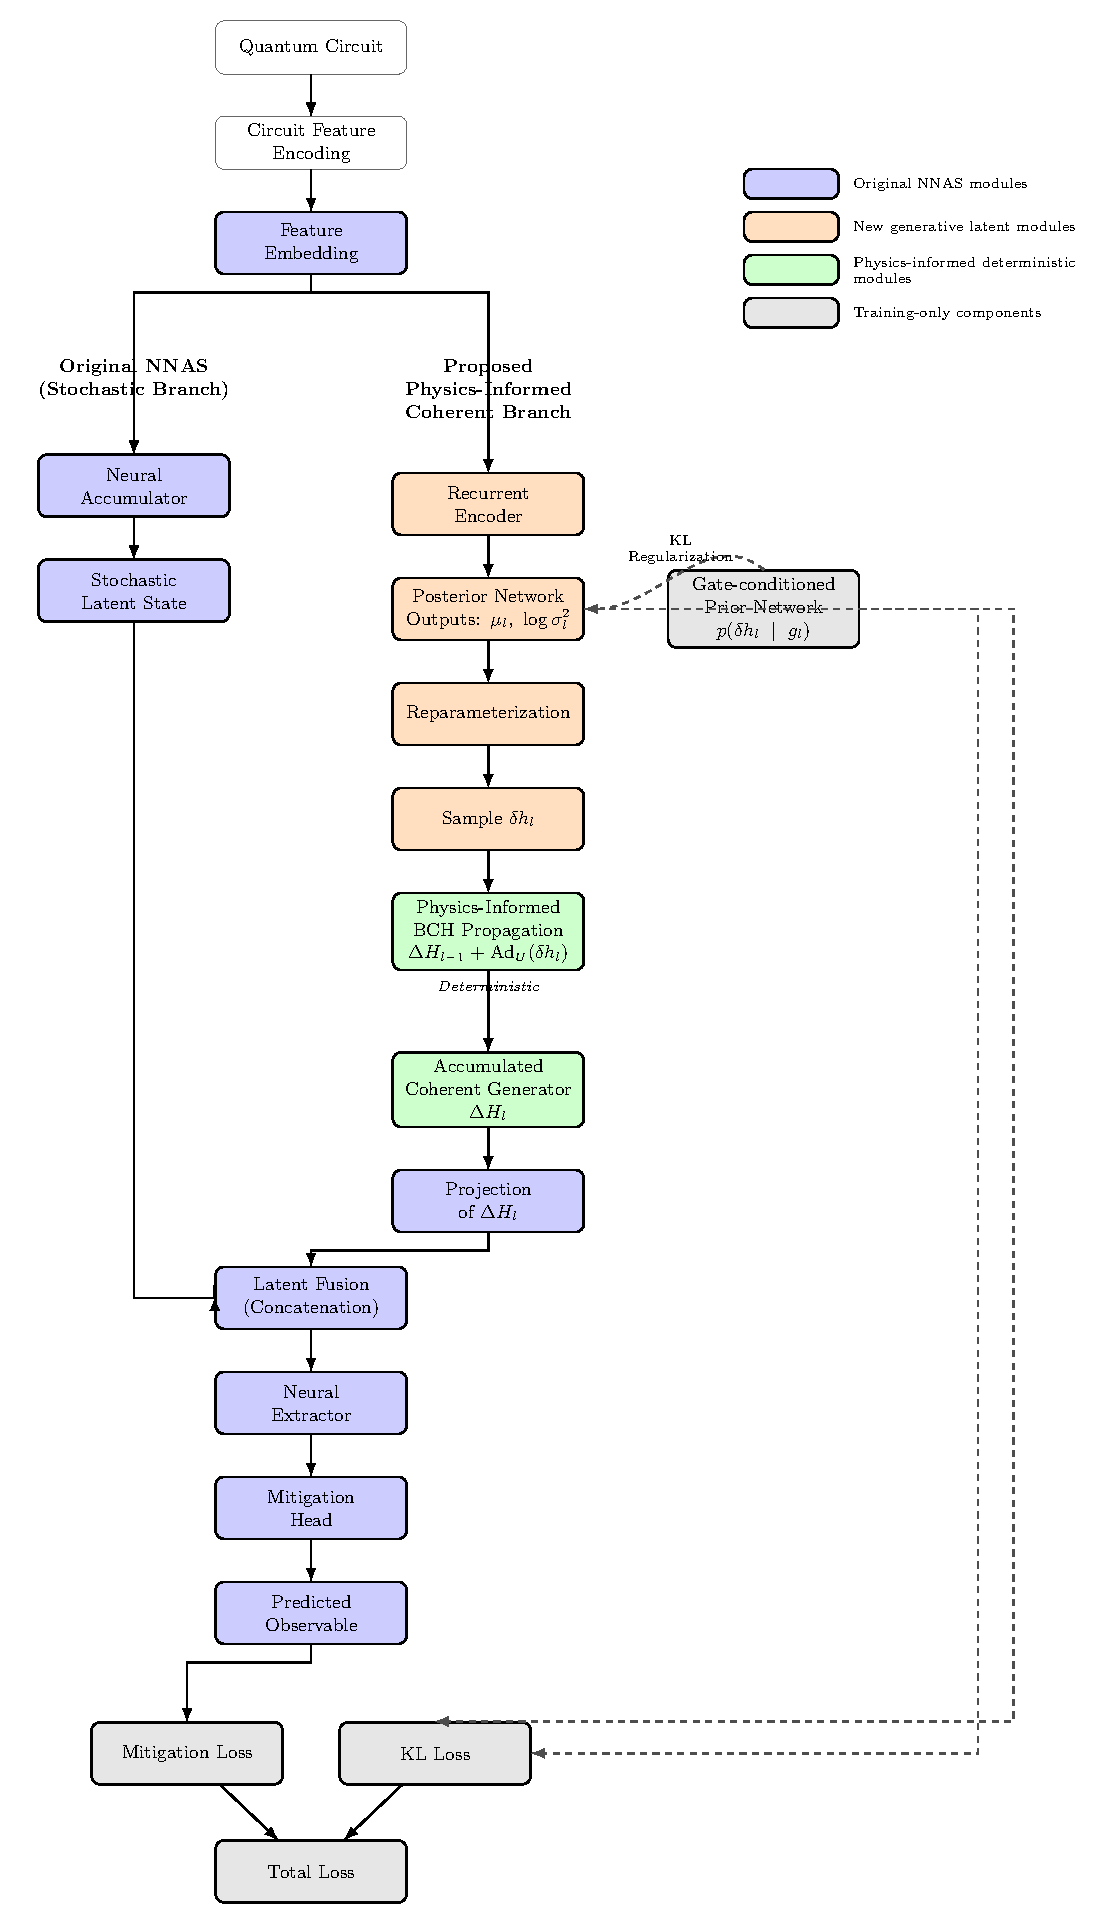
\includegraphics[scale=0.62]{flowchart.pdf}
    \caption{Proposed extension of the NNAS architecture. The original stochastic branch is preserved, while a new conditional generative coherent branch estimates local coherent error generators. These generators are propagated through a deterministic BCH-inspired module before being fused with the stochastic latent representation. During training, a gate-conditioned prior regularizes the latent coherent generators through a Kullback--Leibler divergence, while inference relies solely on the learned posterior and the physics-informed propagation module.}
    \label{fig:nnas-architecture}
\end{figure*}